%%%%%%%%%%%%%%%%%%%%%%%%%%%%%%%%%%%%%%%%%
% Stylish Curriculum Vitae
% LaTeX Template
% Version 1.1 (September 10, 2021)
%
% This template originates from:
% https://www.LaTeXTemplates.com
%
% Authors:
% Stefano (https://www.kindoblue.nl)
% Vel (vel@LaTeXTemplates.com)
%
% License:
% CC BY-NC-SA 4.0 (https://creativecommons.org/licenses/by-nc-sa/4.0/)
%
%%%%%%%%%%%%%%%%%%%%%%%%%%%%%%%%%%%%%%%%%
% !TEX program = xelatex
\documentclass[a4paper, oneside, final, 12pt]{scrartcl} % Paper options using the scrartcl class

\usepackage{fontspec} % for other font
\usepackage{xeCJK} % for chinese font
\usepackage{hyperref} % for hyper web link
\usepackage{multirow} % for tabular table in learning progress
\usepackage{graphicx} % for image insersion
\usepackage[export]{adjustbox} % for image frame
\usepackage{setspace}
\usepackage{array}
% Define typographic struts, as suggested by Claudio Beccari
%   in an article in TeX and TUG News, Vol. 2, 1993.
\usepackage{mathptmx}
\usepackage{scrlayer-scrpage} % Provides headers and footers configuration
\usepackage{titlesec} % Allows creating custom \section's
\usepackage{marvosym} % Allows the use of symbols
\usepackage{tabularx,colortbl} % Advanced table configurations
% \usepackage{ebgaramond} % Use the EB Garamond font
\usepackage{microtype} % To enable letterspacing
\usepackage{pdfpages} % for showing pdf
\usepackage{pdflscape}
\usepackage{enumitem}
\usepackage{subcaption}
\usepackage{listings}   % highlight the python code
\usepackage{xcolor}
\usepackage{multirow}
\usepackage{cite} %Imports biblatex package
\usepackage[ruled,linesnumbered]{algorithm2e}
\newcommand\mycommfont[1]{\normalsize\ttfamily\textcolor{blue}{#1}}
\SetCommentSty{mycommfont}
% \usepackage[backend=bibtex,bibencoding=ascii,style=authoryear,sorting=none]{bibtex}
% \addbibresource{reference.bib}
% setup the margin
\usepackage[top=1cm, bottom=1cm, right=2cm, left=2cm]{geometry}

% set the style of listing code
\definecolor{codegreen}{rgb}{0,0.6,0}
\definecolor{codegray}{rgb}{0.5,0.5,0.5}
\definecolor{codepurple}{rgb}{0.58,0,0.82}
\definecolor{backcolour}{rgb}{0.95,0.95,0.92}

\lstdefinestyle{mystyle}{
    backgroundcolor=\color{backcolour},   
    commentstyle=\color{codegreen},
    keywordstyle=\color{magenta},
    numberstyle=\tiny\color{codegray},
    stringstyle=\color{codepurple},
    basicstyle=\ttfamily\footnotesize,
    breakatwhitespace=true,         
    breaklines=true,                 
    captionpos=b,                    
    keepspaces=true,                 
    numbers=left,                    
    numbersep=5pt,                  
    showspaces=false,                
    showstringspaces=false,
    showtabs=false,                  
    tabsize=2
}

\lstset{style=mystyle}

% set chinese and english font
\setmainfont{Times New Roman}
\setCJKmainfont[AutoFakeBold=true, AutoFakeSlant=true]{標楷體}

\titleformat{\section}{\Large\raggedright\bfseries}{}{0em}{}[\titlerule] % Section formatting
\titleformat{\subsection}{\large\raggedright\bfseries}{}{0em}{}
\titleformat{\subsubsection}{\normalsize\raggedright\bfseries}{}{0em}{}

% \pagestyle{scrheadings} % Print the headers and footers on all pages

% enable bold and slant chinese font
% \xeCJKsetup{AutoFakeBold=true, AutoFakeSlant=true}

% set the space at the front of paragraph
\setlength{\parindent}{2em}

% disable page number
\pagenumbering{gobble}

\newcommand{\gray}{\rowcolor[gray]{.90}} % Custom highlighting for the work experience and education sections
\newcommand{\Tstrut}{\rule{0pt}{2.6ex}}         % = `top' strut
\newcommand{\Bstrut}{\rule[-0.9ex]{0pt}{0pt}}   % = `bottom' strut
\newcommand{\Tstruth}{\rule{0pt}{4ex}}         % = `top' strut for header
\newcommand{\Bstruth}{\rule[-2.5ex]{0pt}{0pt}}   % = `bottom' strut for header

%----------------------------------------------------------------------------------------
%	FOOTER SECTION
%----------------------------------------------------------------------------------------

% \renewcommand{\headfont}{\normalfont\rmfamily\scshape} % Font settings for footer

% \cofoot{
% \fontsize{12.5}{17}\selectfont % Letter spacing and font size

% \textls[150]{123 Broadway {\large\textperiodcentered} City {\large\textperiodcentered} Country 12345}\\ % Your mailing address
% {\Large\Letter} \textls[150]{john@smith.com \ {\Large\Telefon} (000) 111-1111} % Your email address and phone number
% }

%----------------------------------------------------------------------------------------
\begin{document}

%----------------------------------------------------------------------------------------
%	HEADER SECTION
%----------------------------------------------------------------------------------------


\begin{center}
    {\fontsize{18}{30}\textbf{NYCU 2023 Autumn \\ Data Vislualization \\ Final Project Report Team23}} \\
\end{center}

% list two authors information side by side
  \begin{minipage}[t]{0.45\textwidth}
    \begin{center}
      \textbf{Bo-Han Chen (陳柏翰)} \\
      Student ID: 312551074 \\
      bhchen312551074.cs12@nycu.edu.tw
    \end{center}
  \end{minipage}
  \begin{minipage}[t]{0.45\textwidth}
    \begin{center}
      \textbf{Xu Lin (林煦)} \\
      Student ID: 312553027 \\
      f94061042.cs12@nycu.edu.tw
    \end{center}
  \end{minipage}

\section{Abstract}

  In this project, we develop a data vislualization system for
  raffic accident data in Taiwan in 2022.
  Our goal is to find out several insights
  related to the cause and trend of traffic accident,
  which can help the experts and government to improve traffic safety.
  With our system, the user can easily find out the temporal and spatial trend of the accident,
  additionally, the driver-contributed cause and vehicle information 
  are also included, which can be used for further analysis.

\section{Motivation}

  Since there are many people injured or killed in traffic accidents every year,
  so the analysis of the traffic accident data 
  is important and necessary to prevent the accident.
  Some of the accidents are caused by the driver's behavior,
  and some are caused by the road condition 
  and the circumstance such as weather condition at the time that the accident happened.
  Therefore, an easy-to-understand data vislualization 
  can help the experts to analyze the cause of the accident
  and promote the right policy to drivers and pedestrians.
  By analyzing the circumstance of the accident,
  we can also find the dangerous road condition and time period,
  which can help the government to decrease the accident rate 
  by improving the road condition and employing more traffic police at the certain time period.
  
  \subsection{Questions to Answer}
  
  The following questions are what we want to answer by visualizing the dataset.
  
  \begin{enumerate}
    \item Which time period has the highest accident rate?
    \item Which weather condition mainly causes the accident?
    \item Is there any relationship between the 
    driver-contributed causes and the type of vehicle?
    \item Which part of the vehicle is most likely to be hit and fragile during the crash?
  \end{enumerate}

\section{Dataset}

\begingroup
\raggedright

The dataset we choose is the Taiwan road traffic accident statistics 
in 2022 (\emph{111年傷亡道路交通事故資料}), which contains the details of
the accidents that cause death or injury in Taiwan.
The dataset is public and can be accessed from Open Data Website of Taiwan Government
\footnote{\url{https://data.gov.tw/dataset/161199}.}.

\subsection{Data Description}

The dataset contains 845547 records, 
including 4544 A1 level records and 841003 A2 records.
The A1 level means the accident causes death in within 24 hours,
and the A2 level means the accident causes injury or death in more than 24 hours.
Each record contains 51 attributes, including the time, location,
weather, road type, vehicle type, and the number of death/injury.
Some details such as whether the driver is drunk or not, 
which part of the vehicle hit in the accident, 
and the driver-contributed cause of the accident are also included.

\section{Methodology}

Figure \ref{fig: system_overview} shows the overview of our vislualization system.
The system is devided into 6 parts,
including Taiwan traffic accident map, line chart of death / injury trend, 
stream chart of death / injury trend on different weather condition,
heatmap of accident rate, stacked bar chart of driver-contributed cause and vehicle type,
and the crash position distribution of vehicle.

\begin{figure}[htbp]
  \centering
  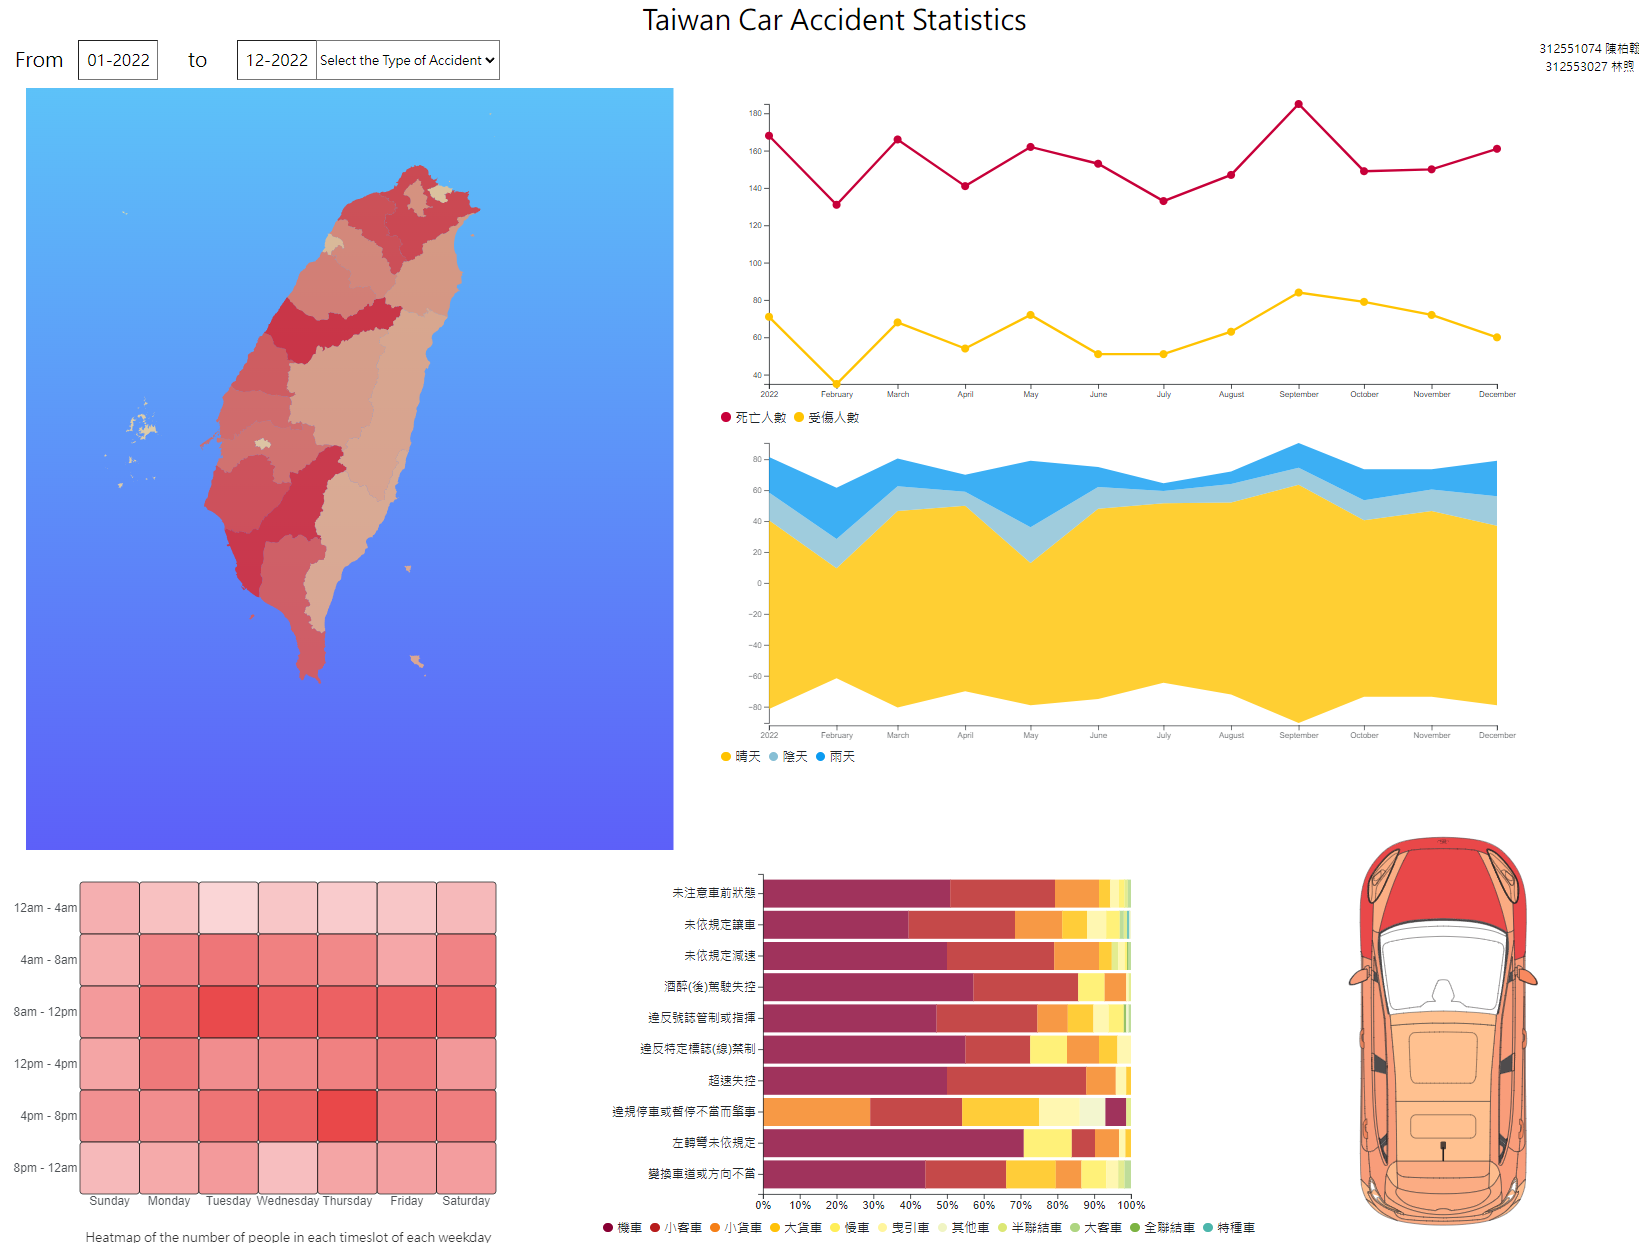
\includegraphics[width=1\textwidth]{"./Image/system_overview.png"}
  \caption{System Overview}
  \label{fig: system_overview}
\end{figure}

\subsection{Taiwan Traffic Accident Map}

This map shows the death / injury count of each cities in Taiwan.
The user can directly indicate which city has high fatality counts 
in the selected time period with the ordinal color scheme.
For detailed information, the user can move the mouse to the city
and the tooltip will show the death / injury count,
drunk driver count, and the mobile phone usage count,
which shows in Figure \ref{fig: map_tooltip}.

\begin{figure}[htbp]
  \centering
  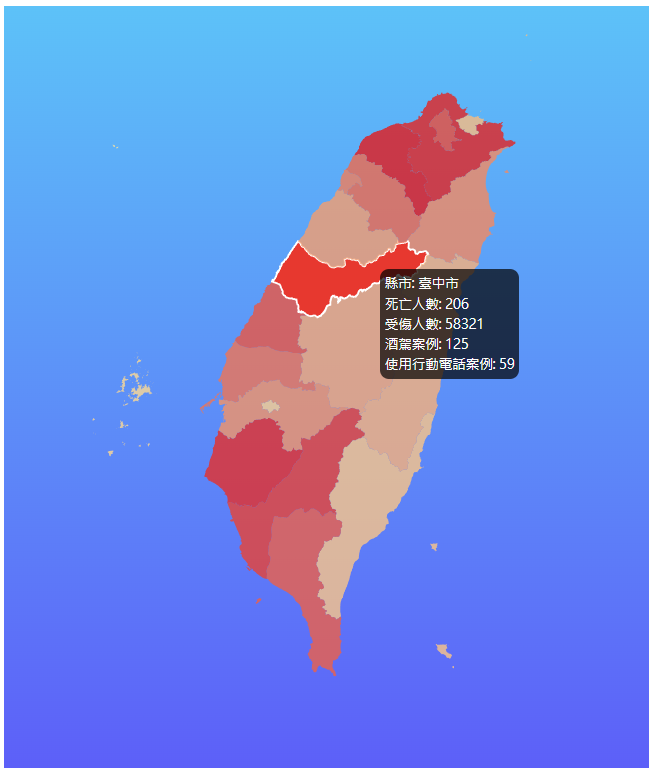
\includegraphics[width=0.6\textwidth]{"./Image/map_tooltip.png"}
  \caption{Map Tooltip}
  \label{fig: map_tooltip}
\end{figure}

\subsection{Line Chart of Death / Injury Trend}

This line chart shows the death / injury trend in the selected time period,
which can help the user to find out the temporal trend of the accident.
The chart will also show fine-grained information when the selected time period is small,
For example, if the user selects the time period of 1 month,
the chart will show the trend of each day in the selected month,
if the selected period is larger than 1 month,
the chart will show the weekly trend.
The tooltip shows the time period and death / injury count of each data point,
which shows in Figure \ref{fig: line_tooltip}.

\begin{figure}[htbp]
  \centering
  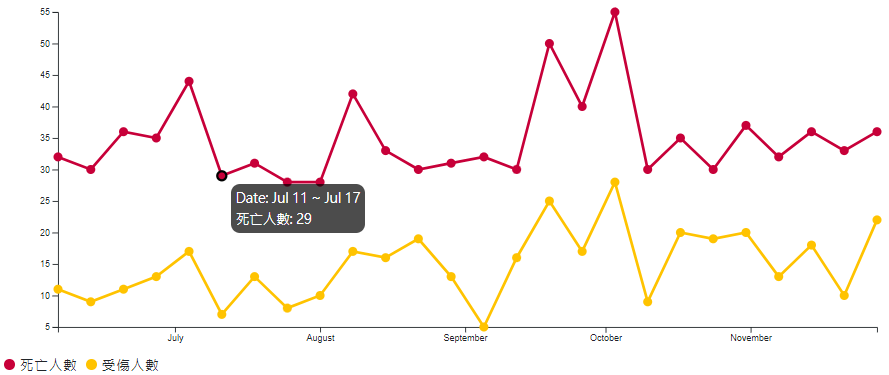
\includegraphics[width=1.0\textwidth]{"./Image/line_tooltip.png"}
  \caption{Line Chart Tooltip}
  \label{fig: line_tooltip}
\end{figure}

\subsection{Stream Chart of Accident Count on Different Weather Condition}

This stream chart shows the accident count on different weather condition.
User can find out the accident trend on different weather condition.
The weather condition is divided into 3 categories,
including sunny, cloudy, and rainy.
Figure \ref{fig: stream_tooltip} shows the stream chart in our system,
the tooltip shows the time period and accident count on different weather condition.

\begin{figure}[htbp]
  \centering
  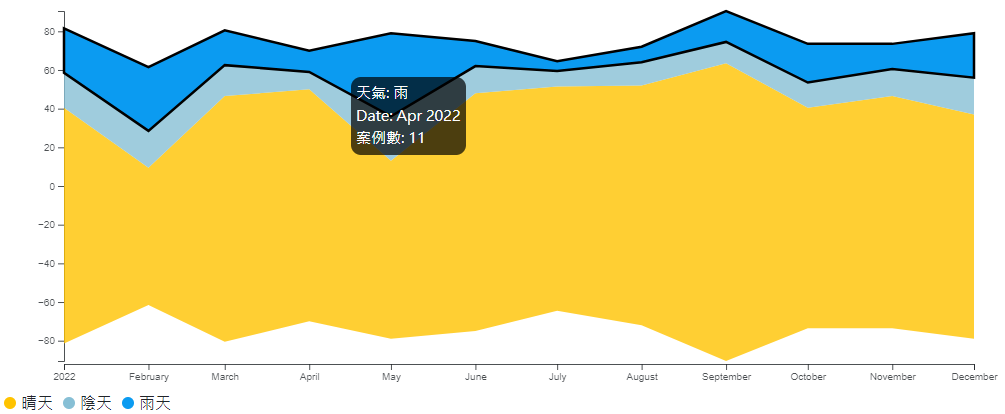
\includegraphics[width=1.0\textwidth]{"./Image/stream_tooltip.png"}
  \caption{Stream Chart Tooltip}
  \label{fig: stream_tooltip}
\end{figure}

\subsection{Grid Heatmap of Accident Count}

The heatmap shows the accident count by time of day and day of week.
This helps user to find out the cyclical trend of the accident,
such as comparing the accident count between weekday and weekend,
and the accident count in the morning and afternoon.
Figure \ref{fig: heatmap_tooltip} shows the heatmap in our system,
the tooltip shows the time period and accident count of each cell.

\begin{figure}[htbp]
  \centering
  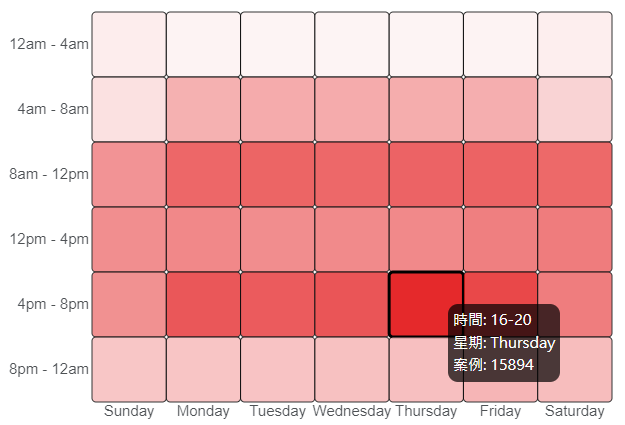
\includegraphics[width=0.7\textwidth]{"./Image/heatmap_tooltip.png"}
  \caption{Heatmap Tooltip}
  \label{fig: heatmap_tooltip}
\end{figure}

\subsection{Stacked Bar Chart of Driver-Contributed Cause and Vehicle Type}

This stacked bar chart shows the ratio of vehicle type for each driver-contributed cause.
User can first find out the frequent driver-contributed cause,
which is sorted by the total accident count.
Then, user can find out the vehicle type that is 
most likely to be involved in the corresponding cause.
Figure \ref{fig: stacked_tooltip} shows the stacked bar chart in our system,
on this chart, we can find out that the most frequent cause is
"未注意車前狀態", and the tooltip shows that scooter is the most likely vehicle type
to be involved in this cause, which is 50.9\% of the total accident count.

\begin{figure}[htbp]
  \centering
  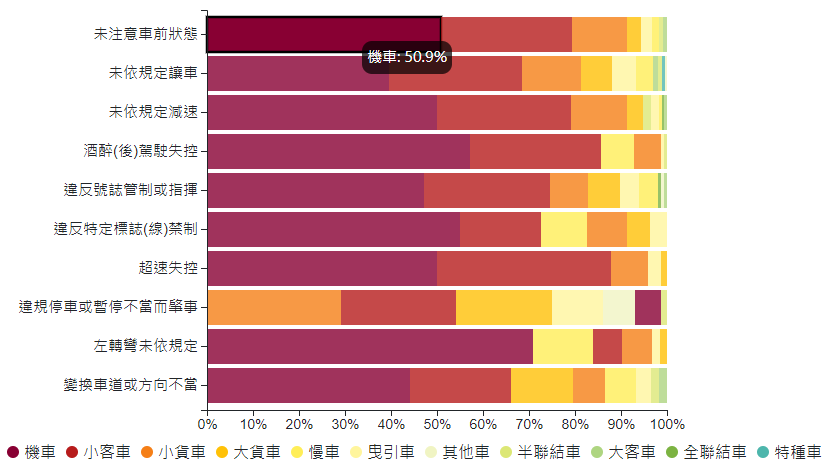
\includegraphics[width=0.8\textwidth]{"./Image/stacked_tooltip.png"}
  \caption{Stacked Bar Chart Tooltip}
  \label{fig: stacked_tooltip}
\end{figure}

\subsection{Crash Position Distribution of Vehicle}

This chart shows the crash position distribution of vehicle.
In our dataset, the crash position is divided into 8 categories,
including front, rear, left, right, front-left, front-right, rear-left, and rear-right.
User can find out which part of the vehicle is most likely to be hit
and fragile during the crash by the ordinal color scheme.
Figure \ref{fig: crash_tooltip} shows the crash position distribution of vehicle in our system,
the tooltip shows the crash position and the accident count.

\begin{figure}[htbp]
  \centering
  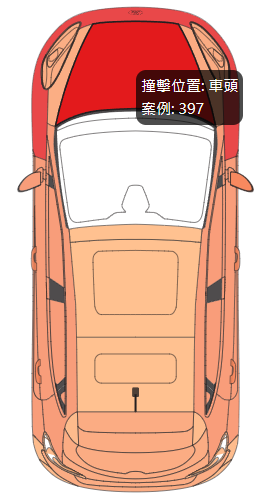
\includegraphics[width=0.3\textwidth]{"./Image/crash_tooltip.png"}
  \caption{Crash Position Distribution of Vehicle Tooltip}
  \label{fig: crash_tooltip}
\end{figure}

\subsection{Interaction}

The user can select the time period and type of accident data (A1, A2, or both)
in the control panel on top of the system (Figure \ref{fig: control_panel}).
Furthermore, city selection is also available in the map,
by clicking the city, system will show the corresponding information.

\begin{figure}[htbp]
  \centering
  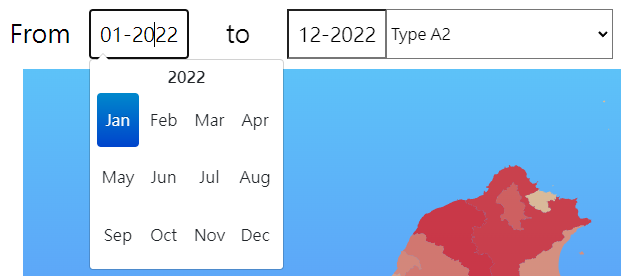
\includegraphics[width=0.8\textwidth]{"./Image/panel.png"}
  \caption{Control Panel}
  \label{fig: control_panel}
\end{figure}

\section{Insights}

\subsection{Temporal \& Spatial Trend}

By selecting both A1 and A2 data, we can first find out the city
that has the high fatality and injury count in 2022 is New Taipei City,
TaoYuan City, Taichung City, and Tainan City in Figure \ref{fig: insight_trend_map}.
each of them has more that 58000 injury count and 160 death count.
Comparing the casualty count between different cities in Taiwan,
we can find out that the count in eastern Taiwan is much lower than the other cities,
which we can infer is because the traffic density is lower in eastern Taiwan.

\begin{figure}[htbp]
  \centering
  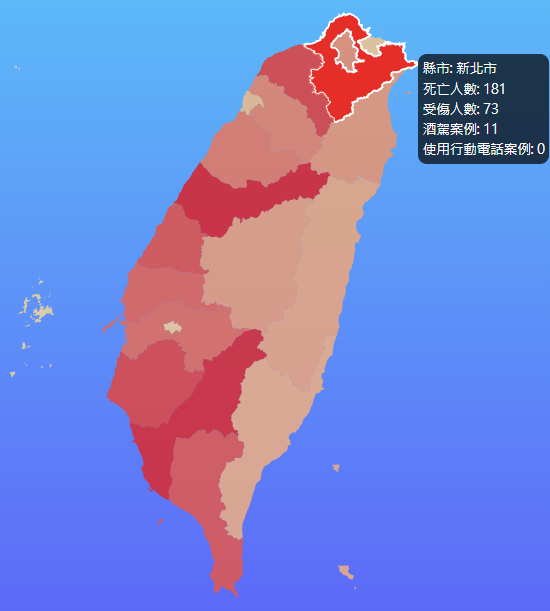
\includegraphics[width=0.5\textwidth]{"./Image/insight_trend_map.png"}
  \caption{Accident Trend in Different City}
  \label{fig: insight_trend_map}
\end{figure}

We can further find out the accident trend in eastern / western Taiwan.
By selecting eastern cities such as Taitung, 
we can find out that the peak of the accident count
is in july and August from Figure \ref{fig: taitung_line},
and the accident count on weekend is abnormaly high shown in Figure \ref{fig: taitung_heatmap}.
We infer that the reason is there are many tourists in eastern Taiwan during summer vacation,
and the traffic density will increase during the weekend, 
which causes more accident than other time period.

% two figures side by side
\begin{figure}[htbp]
  \centering
  \begin{subfigure}[b]{0.6\textwidth}
      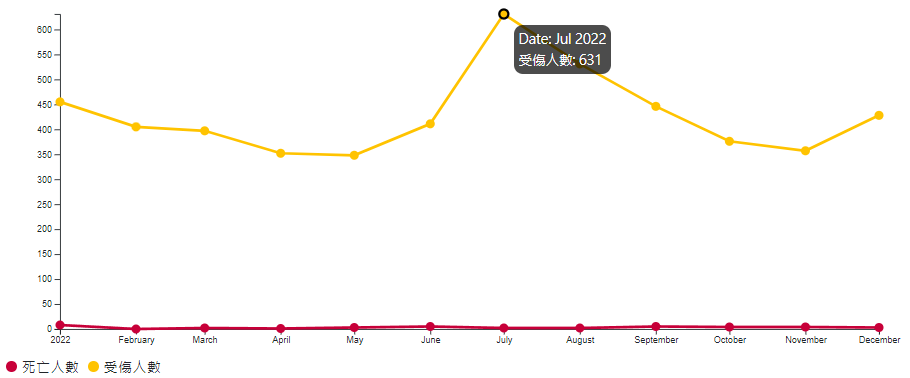
\includegraphics[width=\textwidth]{"./Image/eastern_line.png"}
      \caption{Accident Trend in Taitung}
      \label{fig: taitung_line}
  \end{subfigure}
  \begin{subfigure}[b]{0.35\textwidth}
      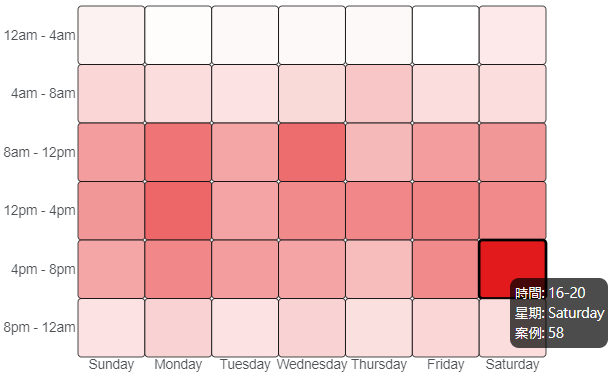
\includegraphics[width=\textwidth]{"./Image/eastern_heatmap.png"}
      \caption{Accident Count in Taitung}
      \label{fig: taitung_heatmap}
  \end{subfigure}
  \caption{Accident Trend in Taitung}
  \label{fig: taitung}
\end{figure}

For western cities such as Hsinchu,
the trend can be found in Figure \ref{fig: hsinchu}.
We can find out that the casualty count becomes 
higher in winter from Figure \ref{fig: hsinchu_line},
this may cause by the early sunset and rainy weather in winter.
From Figure \ref{fig: hsinchu_heatmap}, we can notice that
the accident count is higher in the 8:00-12:00 and 16:00-20:00,
which is the time period that people go to work and go home,
so the traffic density is higher than other time period,
which causes more accident.
Furthermore, the accident count on Friday in period of 16:00-20:00
is higher than other weekday, we think the reason is that
people may go to other city for travel or go back to their hometown
during the weekend, so the traffic density is higher than other weekday.

\begin{figure}[htbp]
  \centering
  \begin{subfigure}[b]{0.6\textwidth}
      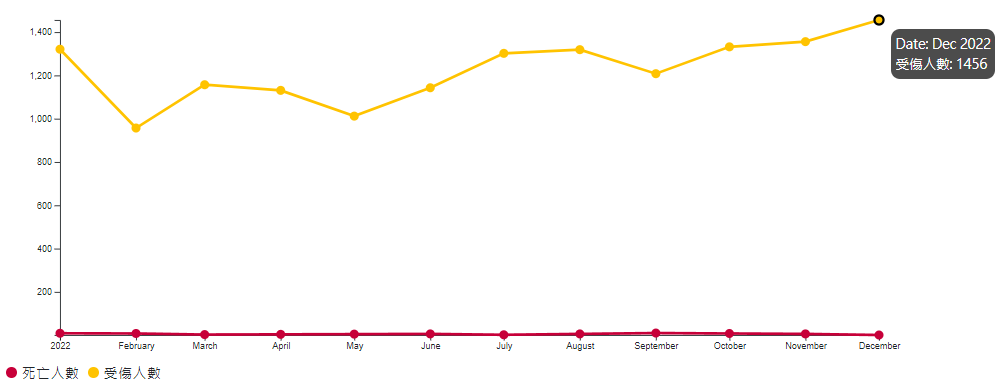
\includegraphics[width=\textwidth]{"./Image/western_line.png"}
      \caption{Accident Trend in Hsinchu}
      \label{fig: hsinchu_line}
  \end{subfigure}
  \begin{subfigure}[b]{0.35\textwidth}
      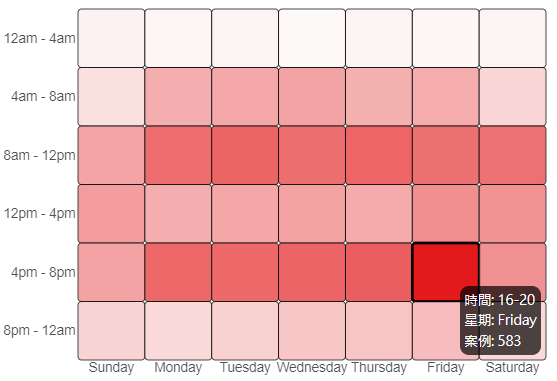
\includegraphics[width=\textwidth]{"./Image/western_heatmap.png"}
      \caption{Accident Count in Hsinchu}
      \label{fig: hsinchu_heatmap}
  \end{subfigure}
  \caption{Accident Trend in Hsinchu}
  \label{fig: hsinchu}
\end{figure}

% \subsection{Color Selection}

% For cartography color selection, 
% we use the colorbrewer2\footnote{\url{https://colorbrewer2.org/}.}
% to select the color scheme for our map.
% For ordered data, we choose the viridis color scheme,
% which is colorblind-friendly and perceptually uniform.

\endgroup

% \bibliographystyle{unsrt} % We choose the "plain" reference style
% \bibliography{reference} % Entries are in the "references.bib" file

\end{document}